% =====================================================================
% AI Academy -- National AI Center
% Software Engineering Final Project -- Team Presentation Deck
% Topic 4 -- Async Research Assistant
%
% Built from templates/SLIDES_TEMPLATE.tex. Compile with pdfLaTeX.
% A PowerPoint rendering of the same 11 slides is slides/slides.pptx.
% Remaining red [TODO: ...] markers: team name, members B/C, live
% benchmark numbers.
% =====================================================================

\PassOptionsToPackage{dvipsnames}{xcolor}
\documentclass[aspectratio=169,11pt]{beamer}

% ===== EARLY MACROS ==================================================
\definecolor{accent2}{HTML}{8B0000}
\newcommand{\TODO}[1]{\textcolor{accent2}{\textbf{[TODO: #1]}}}

% ===== CONFIGURATION =================================================
\newcommand{\teamname}{\TODO{Team Name}}
\newcommand{\topicchoice}{Topic 4 -- Async Research Assistant}
\newcommand{\memberone}{Sanan Garibli}
\newcommand{\membertwo}{\TODO{Member B}}
\newcommand{\memberthree}{\TODO{Member C}}
\newcommand{\repolink}{github.com/sanan-garibli/research-assistant}

\newcommand{\coursecode}{AI-ENG-110}
\newcommand{\coursename}{Software Engineering}
\newcommand{\institution}{AI Academy, National AI Center}
\newcommand{\semester}{Spring 2026}

% ===== PACKAGES ======================================================
\usepackage[T1]{fontenc}
\usepackage[utf8]{inputenc}
\usepackage{xcolor}
\usepackage{tabularx}
\usepackage{booktabs}
\usepackage{listings}
\usepackage{tikz}
\usetikzlibrary{shapes.geometric,arrows.meta,positioning,fit,backgrounds}

% ===== BEAMER THEME ==================================================
\usetheme{default}
\usefonttheme{professionalfonts}
\setbeamertemplate{navigation symbols}{}

\definecolor{accent}{HTML}{0B3D91}
\definecolor{soft}{HTML}{F2F4F8}
\definecolor{ok}{HTML}{166534}

\setbeamercolor{title}{fg=accent}
\setbeamercolor{frametitle}{fg=accent}
\setbeamercolor{section in head/foot}{bg=accent,fg=white}
\setbeamercolor{itemize item}{fg=accent}
\setbeamercolor{itemize subitem}{fg=accent}
\setbeamercolor{enumerate item}{fg=accent}
\setbeamercolor{block title}{bg=accent,fg=white}
\setbeamercolor{block body}{bg=soft,fg=black}

\setbeamerfont{title}{size=\Large,series=\bfseries}
\setbeamerfont{frametitle}{size=\large,series=\bfseries}
\setbeamerfont{footline}{size=\tiny}

\setbeamertemplate{footline}{%
  \leavevmode%
  \hbox{\hspace*{2ex}\tiny\textit{\teamname{} -- \topicchoice}\hfill%
  \tiny\textit{\coursecode{} -- \semester{}}\hfill%
  \tiny\insertframenumber/\inserttotalframenumber\hspace*{2ex}}%
  \vskip1pt%
}

% ===== CODE LISTINGS =================================================
\definecolor{codegreen}{rgb}{0,0.55,0}
\definecolor{codepurple}{rgb}{0.55,0,0.78}
\lstdefinestyle{python}{
  language=Python,
  backgroundcolor=\color{soft},
  commentstyle=\color{codegreen},
  keywordstyle=\color{accent},
  stringstyle=\color{codepurple},
  basicstyle=\ttfamily\scriptsize,
  breaklines=true,
  frame=single,
  framerule=0.4pt,
  rulecolor=\color{black!30},
  showstringspaces=false,
}

% =====================================================================
\begin{document}

% ========== SLIDE 1: TITLE ===========================================
{%
\setbeamertemplate{footline}{}
\begin{frame}[plain]
  \begin{center}
    \vspace{0.6cm}
    {\small \textsc{\institution}}\\[0.2em]
    {\small \textsc{\coursecode{} -- \coursename{} -- \semester{}}}\\[1.2em]
    \rule{0.7\textwidth}{0.6pt}\\[0.4em]
    {\Huge\bfseries\color{accent} \topicchoice}\\[0.4em]
    \rule{0.7\textwidth}{0.6pt}\\[1.2em]
    {\large \teamname}\\[0.6em]
    {\normalsize \memberone\quad\textbullet\quad\membertwo\quad\textbullet\quad\memberthree}\\[1cm]
    {\footnotesize\itshape Final Project Defense -- 11 September 2026}\\[0.4em]
    {\footnotesize\texttt{\repolink}}
  \end{center}
\end{frame}
}

% ========== SLIDE 2: PROBLEM =========================================
\begin{frame}{The problem in one sentence}
  \begin{block}{What the system does}
    A user asks a research question from the command line; we query Wikipedia, arXiv and a web-search API \emph{concurrently}, bounded by a per-source timeout, and return one LLM-synthesised paragraph whose every claim carries a numbered citation --- even when one of the three sources is down.
  \end{block}

  \vspace{0.3em}
  \begin{columns}[T,onlytextwidth]
  \column{0.48\textwidth}
  \textbf{Inputs}
  \begin{itemize}
    \item Question string (trimmed, non-empty, $\le$\,500 chars)
    \item Optional \texttt{--sources wiki,arxiv,web} subset
    \item \texttt{--no-cache} to bypass the source cache
  \end{itemize}

  \column{0.48\textwidth}
  \textbf{Outputs}
  \begin{itemize}
    \item \texttt{ResearchSession}: \texttt{AnswerWithCitations} + one \texttt{SourceOutcome} per source (count, seconds, cache hit, error)
    \item Rendered answer, numbered references with URL, per-source timing line
    \item Exit code 0 (possibly degraded with a note) or 1 with \texttt{Error: ...}
  \end{itemize}
  \end{columns}

  \vspace{0.4em}
  \textbf{Entry points:} \texttt{python -m researcher ask "..."} and \texttt{python -m researcher demo [--limit N]} (no HTTP server; Docker \texttt{CMD} runs the demo).\\
  \textbf{Stack:} Anthropic \texttt{claude-sonnet-5} for synthesis, Tavily for web search, keyless Wikipedia + arXiv.
\end{frame}

% ========== SLIDE 3: ARCHITECTURE ====================================
\begin{frame}{Architecture}
  \textbf{Module map.} One file imports \texttt{ai.*}; one file touches the disk; zero files change to swap Anthropic for OpenAI. {\footnotesize Solid = runtime call, dotted = construction.}

  \vspace{0.1em}
  \begin{center}
  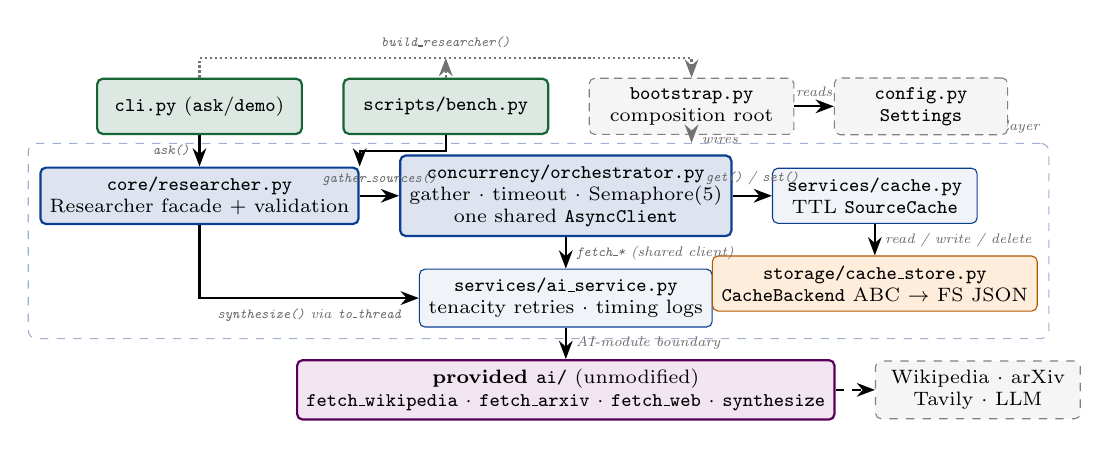
\begin{tikzpicture}[
    node distance=4mm and 5mm,
    box/.style={draw,rounded corners=2pt,minimum width=2.6cm,minimum height=0.7cm,align=center,font=\scriptsize},
    entry/.style={box,fill=ok!15,draw=ok,thick},
    boot/.style={box,fill=black!4,draw=black!50,densely dashed},
    core/.style={box,fill=accent!14,draw=accent,thick},
    svc/.style={box,fill=accent!6,draw=accent},
    store/.style={box,fill=orange!14,draw=orange!70!black},
    aibox/.style={box,fill=violet!10,draw=violet!70!black,thick},
    ext/.style={box,fill=black!4,draw=black!50,dashed},
    arrow/.style={-Stealth,thick},
    wire/.style={-Stealth,densely dotted,thick,black!55},
    lbl/.style={font=\tiny\itshape,text=black!60,align=center}
  ]
    \node[entry] (cli) {\texttt{cli.py} (\texttt{ask}/\texttt{demo})};
    \node[entry,right=of cli] (bench) {\texttt{scripts/bench.py}};
    \node[boot,right=of bench] (boot) {\texttt{bootstrap.py}\\composition root};
    \node[boot,right=of boot,minimum width=2.2cm] (cfg) {\texttt{config.py}\\\texttt{Settings}};

    \node[core,below=of cli] (fac) {\texttt{core/researcher.py}\\Researcher facade + validation};
    \node[core,right=of fac,minimum width=3.6cm] (orch) {\texttt{concurrency/orchestrator.py}\\gather $\cdot$ timeout $\cdot$ Semaphore(5)\\one shared \texttt{AsyncClient}};
    \node[svc,right=of orch] (cache) {\texttt{services/cache.py}\\TTL \texttt{SourceCache}};

    \node[svc,below=of orch] (ais) {\texttt{services/ai\_service.py}\\tenacity retries $\cdot$ timing logs};
    \node[store,below=of cache] (cs) {\texttt{storage/cache\_store.py}\\\texttt{CacheBackend} ABC $\to$ FS JSON};

    \node[aibox,below=of ais,minimum width=5cm] (ai) {\textbf{provided \texttt{ai/}} (unmodified)\\\texttt{fetch\_wikipedia} $\cdot$ \texttt{fetch\_arxiv} $\cdot$ \texttt{fetch\_web} $\cdot$ \texttt{synthesize}};
    \node[ext,right=of ai] (net) {Wikipedia $\cdot$ arXiv\\Tavily $\cdot$ LLM};

    % construction (dotted)
    \draw[wire] (cli.north) -- ++(0,2.5mm) -| node[lbl,above,pos=0.25] {\texttt{build\_researcher()}} (boot.north);
    \draw[wire] (bench.north) -- ++(0,2.5mm);
    \draw[arrow] (boot) -- node[lbl,above] {reads} (cfg);

    % runtime calls (solid)
    \draw[arrow] (cli) -- node[lbl,left] {\texttt{ask()}} (fac);
    \draw[arrow] (bench.south) -- ++(0,-2mm) -| (fac.north east);
    \draw[arrow] (fac) -- node[lbl,above] {\texttt{gather\_sources()}} (orch);
    \draw[arrow] (orch) -- node[lbl,above] {\texttt{get()} / \texttt{set()}} (cache);
    \draw[arrow] (cache) -- node[lbl,right] {read / write / delete} (cs);
    \draw[arrow] (orch) -- node[lbl,right] {\texttt{fetch\_*} (shared client)} (ais);
    \draw[arrow] (fac.south) |- node[lbl,below,pos=0.75] {\texttt{synthesize()} via \texttt{to\_thread}} (ais.west);
    \draw[arrow] (ais) -- node[lbl,right] {AI-module boundary} (ai);
    \draw[arrow,dashed] (ai) -- (net);

    \begin{scope}[on background layer]
      \node[fit=(fac)(orch)(cache)(ais)(cs),draw=accent!40,dashed,rounded corners=3pt,inner sep=4pt,label={[lbl,anchor=south east]north east:\texttt{researcher/} -- our SE layer}] (se) {};
    \end{scope}
    \draw[wire] (boot.south) -- node[lbl,right] {wires} (boot.south |- se.north);
  \end{tikzpicture}
  \end{center}
\end{frame}

% ========== SLIDE 4: KEY DESIGN DECISIONS ============================
\begin{frame}{Three design decisions we can defend}
  \begin{enumerate}\setlength\itemsep{0.6em}
    \item \textbf{asyncio over threads or processes.}\\
      The provided fetchers are coroutines sharing one \texttt{httpx.AsyncClient}; a thread pool would need a loop per thread and lose the shared pool, a process pool cannot pickle the client and there is no CPU work. The one sync call, \texttt{synthesize}, goes through \texttt{asyncio.to\_thread}.
    \item \textbf{One long-lived \texttt{AsyncClient} over a cached SSL context, not one per call.}\\
      Building a client costs $\sim$0.35\,s (trust store). We build it once at composition time, pool connections across questions, and release it with \texttt{async with researcher}. Trade-off accepted: every caller must honour the lifecycle (tests had to be fixed).
    \item \textbf{Filesystem JSON cache behind a \texttt{CacheBackend} ABC, not SQLite/Postgres.}\\
      Payload is small and human-readable; the ABC (like the provided \texttt{WebSearchProvider}) lets tests swap in \texttt{InMemoryCacheBackend}. Multi-process writers or a need for queries over the cache would push us to Postgres.
  \end{enumerate}

  \vspace{0.4em}
  \begin{block}{Expect to be asked}
    ``Why not a \texttt{Protocol} instead of an ABC?'' --- we want a missing \texttt{delete} to fail at construction, not only under mypy.
  \end{block}
\end{frame}

% ========== SLIDE 5: CONCURRENCY (THE BENCHMARK) =====================
\begin{frame}{Concurrency: the benchmark}
  \textbf{Workload:} the 5 sample questions, \texttt{for} loop vs.\ \texttt{asyncio.gather}, \texttt{use\_cache=False} in both phases, fresh client per phase. Command: \texttt{python scripts/bench.py --limit 5}.

  \vspace{0.3em}
  \begin{center}\small
  \begin{tabular}{lcc}
    \toprule
    & \textbf{Sequential} & \textbf{Concurrent (sem=5)} \\
    \midrule
    5 questions, live APIs, wall-clock (s) & \TODO{s} & \TODO{s} \\
    Speedup & 1.0$\times$ & \TODO{$\times$} \\
    1 question, 3 fetches $\times$ 0.2\,s (offline unit benchmark) & 0.60 (sum) & $<0.40$ (measured) \\
    1 question, one source stalls 5\,s, timeout 0.2\,s & 5.05 & $<1.00$ \\
    Provider 429s observed & 0 & 0 \\
    \bottomrule
  \end{tabular}
  \end{center}

  \vspace{0.3em}
  \textbf{Bottleneck named:} per question, $t_{wiki}+t_{arxiv}+t_{web}+t_{llm}$ becomes $\max(t_{wiki},t_{arxiv},t_{web})+t_{llm}$; the LLM call is now the dominant term.\\
  \textbf{What doesn't reach $N\times$:} synthesis is uncached and serialises on the provider's rate limit; \texttt{Semaphore(5)} admits fewer than two questions' fetches at once (chosen for arXiv's $\sim$1\,req/s politeness and Tavily's 1000/month tier).

  \vspace{0.2em}
  {\footnotesize\textit{Live row pending: the report machine sat behind a TLS-intercepting proxy (\texttt{CRYPT\_E\_NO\_REVOCATION\_CHECK} on every host). Numbers reproduce from the README command on an unproxied machine.}}
\end{frame}

% ========== SLIDE 6: ROBUSTNESS STORY ================================
\begin{frame}[fragile]{Robustness: one concrete failure mode}
  \textbf{Scenario:} all three sources fail at once --- first for real (corporate proxy broke TLS to every host), then reproduced with \texttt{PER\_SOURCE\_TIMEOUT\_SECONDS=0.3}.

  \vspace{0.2em}
  \textbf{What the system does:}
  \begin{itemize}\setlength\itemsep{0.2em}
    \item \textbf{Retry:} tenacity, 3 attempts, \texttt{wait\_exponential(0.5\,s $\to$ 8\,s)}, only on \texttt{ProviderError}/\texttt{httpx} errors --- never on \texttt{ValueError}.
    \item \textbf{Bound:} \texttt{asyncio.timeout} per source covers \emph{all} retries; \texttt{gather(return\_exceptions=True)} turns each failure into a \texttt{SourceOutcome.error}.
    \item \textbf{Degrade:} one or two failures $\to$ answer from the rest + \texttt{Note: arxiv unavailable (...)}, exit 0. All three $\to$ \texttt{NoSourcesAvailableError} \emph{before} any LLM spend, exit 1.
  \end{itemize}

  \begin{lstlisting}[style=python,language=bash]
13:47:34,003 WARNING researcher.concurrency.orchestrator: timeout origin=wikipedia after=0.3s
13:47:34,035 WARNING researcher.concurrency.orchestrator: timeout origin=web after=0.3s
13:47:34,036 WARNING researcher.concurrency.orchestrator: timeout origin=arxiv after=0.3s
Error: No sources available for 'What is the current state of fusion energy research?': ['wikipedia', 'arxiv', 'web']
  \end{lstlisting}

  \textbf{What surprised us:} in the real TLS incident the log was \emph{empty} --- the wrapper logs only successes and the gather stores the error text without logging it. Diagnosability gap found; fix queued: \texttt{WARNING} on degraded source + tenacity \texttt{before\_sleep\_log}.
\end{frame}

% ========== SLIDE 7: DEMO ============================================
\begin{frame}[fragile]{Live demo (or scripted demo)}
  \begin{block}{What we will run}
    One hard sample question, cold then warm, inside the Docker image: the second run answers from cache for all three sources and the timing line shows it.
  \end{block}

  \vspace{0.3em}
  \textbf{Demo command (works inside Docker):}
  \begin{lstlisting}[style=python,language=bash]
$ docker build -t research-assistant .
$ docker run --env-file .env research-assistant \
    python -m researcher ask "How does CRISPR-Cas9 gene editing work at a molecular level?"
$ docker run --env-file .env research-assistant \
    python -m researcher ask "how does crispr-cas9 gene editing work at a molecular level?" --sources wiki,arxiv
  \end{lstlisting}

  \vspace{0.3em}
  \begin{itemize}
    \item The answer carries \texttt{[N]} markers and a \texttt{References:} block with \texttt{(origin) title} and URL; hallucinated indices are dropped upstream.
    \item The timing line \texttt{(timing: wikipedia=0.42s, arxiv=0.61s*, ...; * = cache hit)} shows max-not-sum latency and, on the second run, the case-insensitive cache key hitting for every source.
  \end{itemize}

  \vspace{0.2em}
  {\footnotesize\textit{Backup: \texttt{python demo\_ai.py --offline} needs no keys or network and exercises the provided module end to end.}}
\end{frame}

% ========== SLIDE 8: TESTING =========================================
\begin{frame}{Testing}
  \begin{columns}[T,onlytextwidth]
  \column{0.55\textwidth}
  \textbf{Coverage \& shape}
  \begin{itemize}\setlength\itemsep{0.3em}
    \item Total coverage on \texttt{researcher/}: \textbf{95\,\%} (402 stmts, 22 missed)
    \item Provided \texttt{ai/} smoke tests: \textcolor{ok}{\textbf{passing}}, 16/16 unmodified
    \item Test count: \textbf{50 own + 16 smoke = 66}, 1.9\,s
    \item All tests offline; \texttt{ai.*} mocked at our own seam (\texttt{FakeAIService}, \texttt{monkeypatch}) plus the provided \texttt{FakeLLM}
    \item \texttt{mypy researcher}: 0 errors in our code
  \end{itemize}

  \column{0.42\textwidth}
  \textbf{Three tests worth calling out}
  \begin{itemize}\setlength\itemsep{0.3em}
    \item \textbf{Happy path:} CLI \texttt{ask} $\to$ exit 0, answer + references rendered
    \item \textbf{Concurrency:} one source raises, gather degrades; 5\,s stall under 0.2\,s timeout finishes $<1$\,s; semaphore=1 windows never overlap
    \item \textbf{Error path:} the all-sources-fail and partial-failure tests caught the leaked \texttt{AsyncClient} after the shared-client refactor
  \end{itemize}
  \end{columns}

  \vspace{0.6em}
  \begin{block}{Tooling}
    \texttt{pytest} + \texttt{pytest-asyncio} (strict) + \texttt{pytest-cov} + \texttt{unittest.mock}/\texttt{monkeypatch}; \texttt{respx} installed but unused so far. \texttt{mypy researcher --ignore-missing-imports}: 0 errors in \texttt{researcher/} (27 pre-existing in provided \texttt{ai/providers}).
  \end{block}
\end{frame}

% ========== SLIDE 9: LIMITATIONS + FUTURE ============================
\begin{frame}{Limitations \& what we'd do next}
  \textbf{Where the system is brittle today}
  \begin{itemize}\setlength\itemsep{0.3em}
    \item Silent degradation: a failed source's error is stored, not logged; retries are invisible. Worst decision we made.
    \item No 429-aware budget: semaphore is per process, backoff ignores \texttt{Retry-After}; two containers can burn one Tavily key.
    \item Cache is single-writer, lazily expired, never swept; a schema-drifted entry raises and is reported ``unavailable'' until TTL.
    \item Synthesised answers are not cached, so repeated questions always pay the LLM call --- the reason $5\times$ is out of reach.
  \end{itemize}

  \vspace{0.4em}
  \textbf{Given another week we would}
  \begin{enumerate}\setlength\itemsep{0.3em}
    \item Log every retry and degraded source at \texttt{WARNING}; add \texttt{respx} tests for the real fetch path (429, 301, 403).
    \item Cache answers keyed by (question, source URLs, model id); atomic write-then-rename plus a sweeper for the file cache.
    \item Run the live benchmark on an unproxied machine and a 20-question load test; add a \texttt{--json} CLI mode and OpenTelemetry spans.
  \end{enumerate}
\end{frame}

% ========== SLIDE 10: TEAM CONTRIBUTIONS =============================
\begin{frame}{Team contributions}
  \begin{center}\small
  \begin{tabularx}{\linewidth}{lXl}
    \toprule
    \textbf{Member} & \textbf{Primary ownership} & \textbf{Commits} \\
    \midrule
    \memberone   & \texttt{researcher/} SE layer (config, models, services, core, concurrency, storage, CLI), test suite, Dockerfile, benchmark, README, shared-client PR \#1, report \& slides & 100\% (6 of 6 to date) \\
    \membertwo   & \TODO{e.g.\ ownership area}   & \TODO{\%} \\
    \memberthree & \TODO{e.g.\ ownership area}   & \TODO{\%} \\
    \bottomrule
  \end{tabularx}
  \end{center}

  \vspace{0.4em}
  \begin{block}{We can all answer:}
    Any of us can walk through any module on demand. Pick a file --- we'll defend it.
  \end{block}

  \vspace{0.4em}
  \textbf{AI tool use:} Claude Code (Anthropic) drafted the \texttt{researcher/} layer, tests, Dockerfile, README, this report and deck from the topic spec; every file was reviewed by the author, and the User-Agent, redirect and client-lifecycle fixes were made by hand after live failures.
\end{frame}

% ========== SLIDE 11: THANK YOU / Q&A ================================
{%
\setbeamertemplate{footline}{}
\begin{frame}[plain]
  \begin{center}
    \vspace{1cm}
    {\Huge\bfseries\color{accent} Questions?}\\[1.2em]
    \rule{0.5\textwidth}{0.6pt}\\[1.2em]
    {\large \teamname}\\[0.6em]
    {\normalsize \texttt{\repolink}}\\[1cm]
    {\footnotesize\itshape ``We can walk through any file in the repo.''}
  \end{center}
\end{frame}
}

\end{document}
